\section{Matematička formulacija i konceptualni model problema}
\label{chap:model_problema}
Nakon pregleda teorijskih osnova, ovo poglavlje posvećeno je formalnoj definiciji problema optimizacije projektnog portfelja. Cilj je prevesti realni poslovni problem u precizan matematički i konceptualni model na koji se mogu primijeniti računalne metode optimizacije. U nastavku se detaljno opisuju ulazni entiteti, varijable odluke, primijenjena resursna ograničenja te jedno-kriterijski i više-kriterijski ciljevi koji su korišteni u eksperimentalnoj evaluaciji.
\subsection{Definicija skupa aktivnosti i varijabli odluke}
Problem se definira kao odabir optimalnog podskupa (portfelja) aktivnosti iz većeg, unaprijed definiranog skupa dostupnih aktivnosti, što je čest izazov u projektnom menadžmentu \cite{PMI2021, Kerzner2017}. Neka je $A=\{a_1, a_2, ..., a_n\}$ skup od $n$ dostupnih projektnih aktivnosti. Svaka aktivnost $a_i \in A$ opisana je s tri ključna atributa. Prvi je trošak ($c_i$), koji predstavlja količinu budžeta potrebnu za izvođenje aktivnosti. Drugi atribut je vrijednost ($v_i$), definirana kao povrat na investiciju (ROI) koji se ostvaruje uspješnim završetkom. Treći, ključni atribut je nesigurnost trajanja, koja se ne modelira kao jedna deterministička vrijednost, već kao stohastička varijabla opisana s tri točke procjene: optimističnom ($T_o$), najvjerojatnijom ($T_m$) i pesimističnom ($T_p$), koje služe kao parametri za Trokutastu distribuciju u Monte Carlo simulaciji.

S obzirom na navedene atribute, temeljni zadatak optimizacije je definirati binarni vektor odluke $x=(x_1, x_2, ..., x_n)$, gdje $x_i \in \{0,1\}$. Vrijednost $x_i=1$ označava da je aktivnost $a_i$ odabrana za uključivanje u portfelj, dok $x_i=0$ označava da se aktivnost ne izvodi. Ovaj vektor odluke je upravo ono što genetski algoritam nastoji optimizirati.

\subsection{Resursna ograničenja modela}
Iako realni projekti mogu imati višestruka ograničenja, u ovom modelu implementirano je ključno i najčešće ograničenje u upravljanju portfeljem: ograničenje budžeta ($B_{max}$). Prema ovom pravilu, ukupni zbroj troškova svih odabranih aktivnosti ne smije prelaziti ukupno raspoloživi budžet. Formalno, ovo ograničenje odgovara klasičnoj formulaciji problema ruksaka (\textit{Knapsack Problem}) \cite{Kellerer2004} i matematički se izražava kao:
$$
\sum_{i=1}^n c_i x_i \leq B_{max}
$$
Vrijedi napomenuti da ukupno trajanje portfelja nije tretirano kao strogo ograničenje, već kao izlazna metrika performansi i cilj za minimizaciju. Ovakav pristup je fleksibilniji i realističniji, jer menadžerima često nije cilj samo "uklopiti se" u zadani rok, već pronaći portfelj s najboljim mogućim očekivanim trajanjem za određenu razinu povrata na investiciju, što je u skladu s modernim praksama upravljanja projektnom nesigurnošću \cite{Smith2014}.

\subsection{Specifikacija optimizacijskih ciljeva}
U skladu s eksperimentalnim dizajnom, definirana su i analizirana dva različita optimizacijska cilja, što odgovara dvama glavnim testiranim scenarijima.

Prvi, jedno-kriterijski cilj, usmjeren je isključivo na maksimizaciju financijske dobiti. Ovaj pristup odgovara klasičnom GA (samo ROI) modelu, a njegova ciljna funkcija je maksimizacija ukupnog zbroja ROI vrijednosti odabranih aktivnosti, uz poštivanje ograničenja budžeta. Ovakav tip optimizacijskog cilja čest je u primjeni genetskih algoritama na probleme alokacije resursa \cite{Goldberg1989}, a formalno se zapisuje kao:
$$
\max \sum_{i=1}^n v_i x_i
$$
S druge strane, više-kriterijski cilj predstavlja srž ovog istraživanja i odgovara naprednom hibridnom GA+MC (NSGA-II) modelu. U ovom pristupu istovremeno se optimiziraju dva suprotstavljena cilja: (1) maksimizacija ukupnog ROI-a i (2) minimizacija procijenjenog trajanja portfelja. Budući da poboljšanje jednog cilja često degradira drugi, ovaj pristup ne traži jedno jedino "najbolje" rješenje. Umjesto toga, cilj je pronaći skup optimalnih kompromisnih rješenja (tzv. Paretov front), za što je korišten renomirani NSGA-II algoritam \cite{Deb2002}.

\subsection{Konceptualni prikaz modela}
Konceptualni model problema, koji objedinjuje sve prethodno opisane elemente, prikazan je na Slici \ref{fig:konceptualni_model}. Dijagram ilustrira proces u kojem optimizacijski algoritam, kao središnji mehanizam, uzima skup svih dostupnih aktivnosti kao ulaz. Vođen definiranim ciljevima (maksimizacija ROI-a i/ili minimizacija trajanja) i ograničen zadanom budžetom, algoritam pretražuje prostor mogućih kombinacija kako bi kao izlaz generirao optimalni portfelj – podskup aktivnosti koji najbolje zadovoljava postavljene kriterije.

\begin{figure}[H]
    \centering
    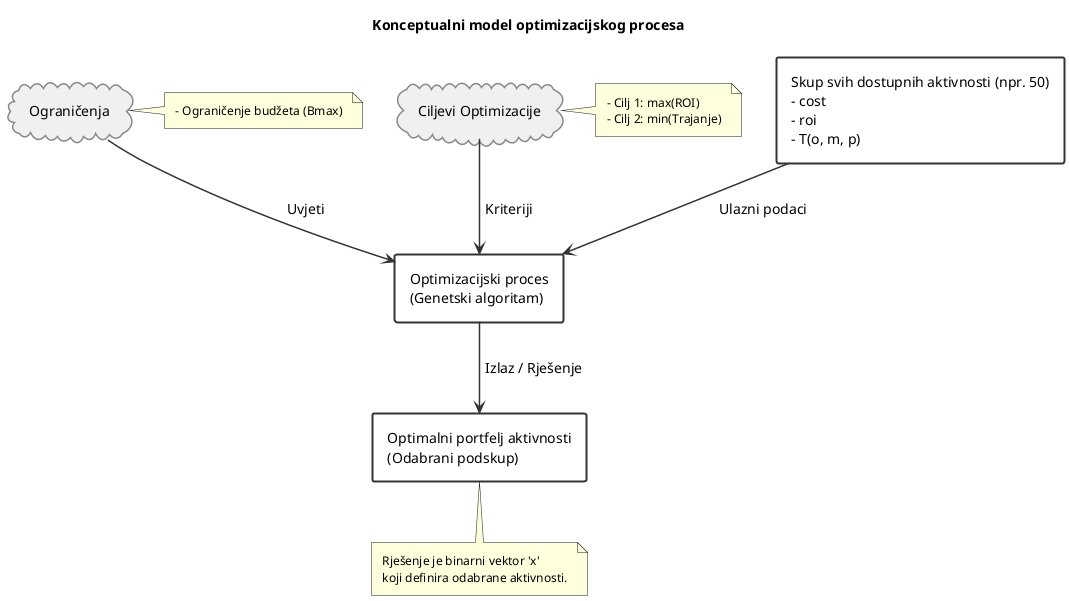
\includegraphics[width=0.8\textwidth]{slike/model_problema.png}
    \caption{Konceptualni model problema optimizacije portfelja projektnih aktivnosti.}
    \label{fig:konceptualni_model}
\end{figure}

Ovaj formalizirani model omogućuje jasnu matematičku i vizualnu reprezentaciju optimizacijskog zadatka. Precizna definicija ulaza, ograničenja i ciljeva ključna je za sustavnu primjenu optimizacijskih metoda poput genetskih algoritama \cite{Mitchell1998} u kombinaciji s Monte Carlo simulacijama \cite{Rubinstein2016}, kako bi se dobila rješenja visoke kvalitete koja su istovremeno i robusna na prisutne nesigurnosti.
